\documentclass{article}
\usepackage{adjustbox}
\usepackage{float}
\usepackage{marvosym}
\usepackage{amsmath}
\usepackage{textcomp}
\usepackage{graphicx}
\graphicspath{{images/}}
\usepackage{booktabs}
\usepackage{color}
\usepackage{verbatim}
\usepackage{listings}
\usepackage{underscore}
\setcounter{secnumdepth}{5}
\usepackage[bookmarks=true]{hyperref}
\author{Roberto Clapis (841859), Erica Stella (854443)} 
\date{\today}
\title{Politecnico di Milano
	\\A.A. 2015\@-\@2016
	\\Software Engineering 2: ``myTaxiService''
	\\\textbf{P}roject \textbf{P}lan}
\hypersetup{pdftitle={Project Plan},    % title
	pdfauthor={Roberto Clapis, Erica Stella},                     % author
	pdfsubject={Project Plan},                        % subject of the document
	pdfkeywords={TeX, LaTeX, taxi, PP, SoftwareEngineering2}, % list of keywords
	colorlinks=true,       % false: boxed links; true: colored links
	linkcolor=black,       % color of internal links
	citecolor=blue,       % color of links to bibliography
	filecolor=black,        % color of file links
	urlcolor=purple,        % color of external links
}
\begin{document}
\maketitle
\begin{center}
	
\includegraphics{polimi-logo}
\end{center}
\clearpage
\tableofcontents
\clearpage
\section{Introduction}
This document describes the project plan for myTaxiService application.
It presents an analysis of the expected size and effort required 
for the implementation phase calculated respectively with the Function
Points and COCOMO\@. Then it presents the available resources and how 
they will be allocated to the project tasks and, in the end, it
discusses the possible risks this project might encounter and the
associated recovery actions.
\section{Size and Effort Estimation}
\subsection{Size Estimation -- Function Points}
Following Albrecht's method, our application's function points
will be divided in 5 types:
\begin{itemize}
	\item Internal Logical File (ILF): homogeneous set of data used
	and managed by the application.
	\item External Interface File (EIF): homogeneous set of data 
	used by the application but generated and maintained by other.
	\item External Input: elementary operation to elaborate data
	coming from the external environment.
	\item External Output: elementary operation that generates data
	for the external environment.
	\item External Inquiry: elementary operation that involves
	input and output.
\end{itemize}
The function points' types stated above will be weighted as 
specified in the following table.
\begin{center}
	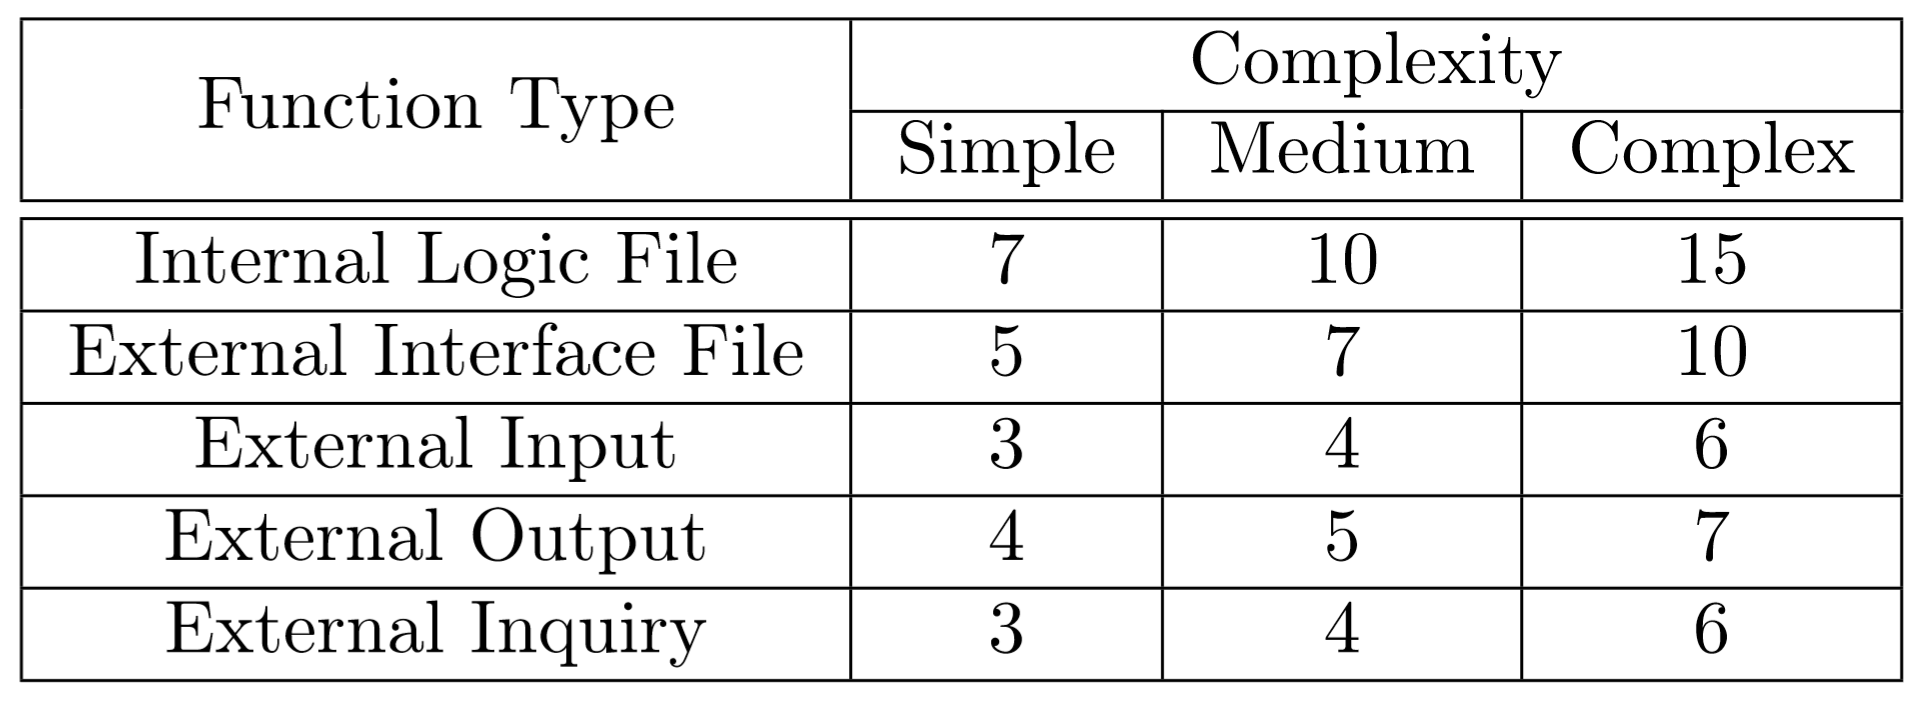
\includegraphics[width = 0.8\textwidth]{FP}
\end{center}
\subsubsection{Internal Logical File}
The application stores information about: 
\begin{itemize}
	\item Admins (user name, password hash, email)
	\item Users (user name, password hash, email)
	\item City zones (nearest zones)
	\item Requests (starting zone, destination zone, taxi code)
	\item Reservations (starting zone, destination zone, taxi code, meeting time)
	\item Taxi drivers (taxi code, user name, password hash, current zone, availability time)
\end{itemize}
The first five entities have a simple structure as they are composed 
of a small number of fields, while the taxi drivers have a more complex
structure that also needs to be updated frequently. Thus we decide to 
adopt the simple weight for the first five and the medium weight
for the last one.
5\texttimes7+1\texttimes10 = 45 FPs concerning ILFs.
\subsubsection{External Interface File}
There are no such things in our project.
\subsubsection{External Input}
myTaxiService application interacts with users
as follows: 
\begin{itemize}
	\item login/logout: as they're simple operations the simple weight can be adopted. 2\texttimes3 = 6 FPs.
	\item registration: this is considered of medium complexity as it requires a careful update of the ILFs. 1\texttimes4 = 4 FPs
	\item request/reserve a taxi: these operations are considered complex as they also involve the calculation of the queues and the CAT. 2\texttimes6 = 12 FPs
	\item cancel a request/reservation: these operation are complex as they involve two entities, users and taxi drivers, and a careful concurrency handling. 2\texttimes6 = 12 FPs
	\item modify personal data: this can be considered of medium complexity as it requires the handling of important information. 4 FPs
	\item toggle taxi driver state: this is considered an easy operation as it concerns only one entity. 3 FPs
	\item accept/refuse requests/reservations: these are considered operations of medium complexity as they require of two important entities. 4\texttimes4 = 16
	\item receiving gps information on the taxi driver's location: this is considered a medium complexity operation. 4 FPs
\end{itemize}
It also interacts with admins as follows:
\begin{itemize}
	\item insert/modify/remove a taxi driver from the database: these can be considered easy operations. 3\texttimes3 = 9 FPs
\end{itemize}
Thus, 70 FPs concerning External Inputs.

\subsubsection{External Output}
The application allows the creation of:
\begin{itemize}
	\item notifications about the taxi code to send to users: we can adopt the simple weight for this operation. 4 FPs
	\item notifications of requests/reservations to send to taxi drivers: we can adopt the simple weight for these operations too. 2\texttimes4 = 8 FPs
	\item notifications of the ETA: this is a complex operation as it involves the calculation of the queues and of the CAT. 7 FPs
\end{itemize}
19 FPs concerning External Outputs.

\subsubsection{External Inquiry}
The application allows users to:
\begin{itemize}
	\item show all his/her active requests and reservations
	\item select a currently active request/reservation
	\item select the street between the available ones
\end{itemize}
and it allows admins to:
\begin{itemize}
	\item show the list of all taxi drivers
	\item select a taxi driver
\end{itemize}
These 6 operations can all be considered easy, so we can adopt the simple weight for all of them. 6\texttimes3 = 18 FPs concerning External Inquiries.

\subsection{Effort Estimation - COCOMO}
%TODO
To convert the function points in SLOC we use a 
conversion factor of 46, as specified here 
http://www.qsm.com/resources/function-point-languages-table
for J2EE.
\begin{center}
	SLOC = FP \texttimes 46 = 152 \texttimes 46 = 6992
\end{center}
We consider our project with all nominal Cost Drivers and
Scale Drivers so we have an EAF of 1.00 and an
exponent E of 1.0997.
\begin{center}
	\EUR ffort = 2.94\texttimes EAF\texttimes $(KSLOC)^{E}$ = 2.94\texttimes$(6.992)^{1.0997}$ = 24.95 Person-Month
\end{center}
The duration of the project could therefore be calculated with the following equation
\begin{center}
	Duration = 3.67\texttimes(\EUR ffort)$^{SE}$ = 3.67\texttimes$24.95^{0.3179}$ = 10.2 months
\end{center}
where SE = 0.3179 as derived from nominal Scale Drivers.
Thus, the estimate of people needed to complete the project is
\begin{center}
	N$_{people}$ = $\frac{Effort}{Duration}$ = 2.45 people $\rightarrow$ 3 people
\end{center}







\section{Resource Allocation}
%TODO descrizione
%TODO ma secondo te dobbiamo farlo cosi'? non dovremmo farlo per il progetto coeme dovessimo fare il codice?
%perchè secondo me non vogliono la distribuzione delle risorse per fare la docuentazione ma epr fare il codice
\subsection{Tasks}
RASD:
\begin{itemize}
	\item Domain assumptions
	\item Functional requirements
	\item Non functional requirements
	\item Use cases and scenarios
	\item User interface
	\item Alloy
\end{itemize}
Design Document:
\begin{itemize}
	\item
\end{itemize}
Code Inspection:
\begin{itemize}
	\item
\end{itemize}
Integration Test Plan Document:
\begin{itemize}
	\item 
\end{itemize}
\section{Risks}
\end{document}
